\section{Extending the methodology in the context of \gls{WCA}}

\todo[inline]{%
    Why do we need to extend the methodology? What was wrong with the approach in the previous section?
}

\subsection{Characterizing human behavior}

\cref{paper:olguinmunoz2021impact} describes a study designed to characterize the effects of system responsiveness on human behavior in step-based \gls{WCA}.
This corresponds to the first step in extending our EdgeDroid tool for the benchmarking of \gls{WCA}, first introduced in \cref{paper:olguinmunoz2018demoscaling,paper:olguinmunoz2019edgedroid}, with a more realistic model of human behavior.

We present in this paper the design and execution of a study in which \num{40} undergraduate students of diverse fields of
study\footnote{%
    Participants were recruited from a pool of students enrolled in an undergraduate psychology course at \gls{CMU}.
}, were asked to interact with and follow the instructions given to them by a \gls{WCA} application.
Unbeknownst to the participants, the system responsiveness of the \gls{WCA} system was systematically altered in real time, and the resulting behavioral and physiological reactions were recorded.

With this study, we intended to answer four core research questions relating to human responses to decreased application responsiveness.
One, do subjects change the temporal profile of their actions in relation to system latency?
We expected this to be the case, although the extent or form of these changes were unknown.
Two, do users show signals of arousal in physiological responses to changes in system latency?
As latency increased and due to the added annoyance of dealing with a less responsive system, we expected users to begin showing signs of stress and frustration.
Three, are responses to delay effects in subjects mediated by cognition and/or emotion?
We expected delay effects in subjects to be mediated primarily by emotion, and in particular expected these effects to be correlated with the level of the reduction in system responsiveness.
And four, are these effects mediated by personality indicators in any way?
It was our hypothesis that, among others, the individual trait of \emph{neuroticism}~\cite{john1999big} would play a particularly important role in mediating effects of reduced system responsiveness on subjects.

\begin{figure}[tb]
    \centering
    \begin{subfigure}[t]{.49\textwidth}
        \centering
        \includegraphics[width=\textwidth]{publications/2021ImpactDelayedResponse/Fig4a}
        \caption{}\label{sfig:regularwcaexec}
    \end{subfigure}%
    \hfill%
    \begin{subfigure}[t]{.49\textwidth}
        \centering
        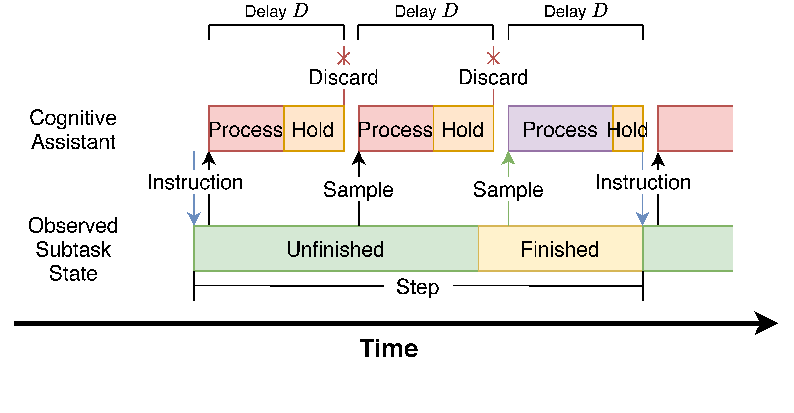
\includegraphics[width=\textwidth]{publications/2021ImpactDelayedResponse/Fig4b}
        \caption{}\label{sfig:delaywcaexec}
    \end{subfigure}
    \caption{%
        Comparison between normal task execution in the LEGO \gls{WCA}~\cite{chen2015early}~(\labelcref{sfig:regularwcaexec}) and modified task execution with delay in the experimental setup of \cref{paper:olguinmunoz2021impact}~(\labelcref{sfig:delaywcaexec}).
        In the experimental task, an additional variable segment of time is introduced immediately following the processing of the input frame in order to extend the perceived processing time of the input to a specific target interval of time denoted \emph{delay}.
    }\label{fig:regularwca-vs-delaywca}
\end{figure}

We employed a version of the step-based \emph{Gabriel} cognitive assistant framework first introduced by \citeauthor{chen2018application}~\cite{chen2018application}.
The assistant was instrumented to capture key application and task performance metrics in real time, in particular step execution time.
Furthermore, the software was modified to allow for the real-time alteration of system responsiveness by extending the processing interval of each input to a temporarily fixed value denoted \emph{delay}.
This is illustrated in \cref{fig:regularwca-vs-delaywca}.
If, during a series of steps, delay was set to a value \ensuremath{\mathbb{D}}, the feedback for each input frame was provided to the user exactly a time interval \ensuremath{\mathbb{D}} after frame capture.
Seven values were selected for \ensuremath{\mathbb{D}}: no added delay (which was referred to as  \SI{0}{\second} delay), \SIlist{0.6;1.125;1.65;2.175;2.7;3.0}{\second}.

\begin{figure}[tb]
    \centering
    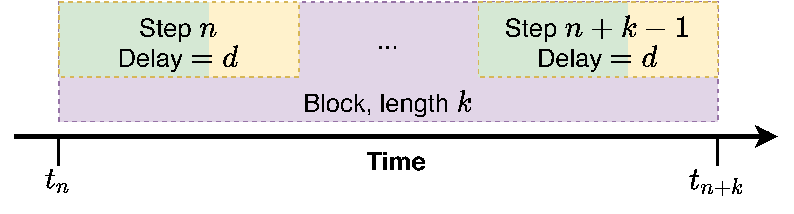
\includegraphics[width=.6\textwidth]{publications/2021ImpactDelayedResponse/Fig4c}
    \caption{Structure of a \emph{block} in the experimental LEGO task.}\label{fig:stepblock}
    \todo[inline]{This figure may need reworking for clarity.}
\end{figure}

The actual \gls{WCA} task employed for this study corresponded to a modified and extended version of the LEGO assembly task introduced in~\cite{chen2015early}.
Unlike the original design of this task, in which the user is led through the assembly of a specific model, the modified LEGO task consisted of a pseudo-random sequence of steps instructing subjects to add or remove pieces.
We introduce an experimental design component denoted a \emph{block}, illustrated in \cref{fig:stepblock}, corresponding to a segment of consecutive steps subject to the same delay value.
To study the effects of a delay applied across multiple steps, we manipulate the length of blocks during the task, using values of \numlist[list-final-separator={, or }]{4;8;12} steps.
We then generate a pseudo-random permutation of the combinations of block length and delay values, and assign a unique sequence of steps to each combination in order to create \num{21} unique blocks of steps.
Using a \emph{Latin-square}~\cite{keedwell2015latin} design, we reorder the initial permutation to generate a task for each of the \num{40} participants.

In order to capture metrics relating to the emotional response of humans to changes in system responsiveness, participants were asked to wear an array of biometric sensors.
This array included devices to capture four physiological measures:
\begin{enumerate*}[itemjoin={{, }}, itemjoin*={{, and }}, label={(\arabic*)}]
    \item \gls{GSR} (also known as electrodermal activity)
    \item accelerometer data from the dominant wrist
    \item brain activity in the form of \gls{EEG}
    \item heart rate
\end{enumerate*}.
Additionally, to measure individual differences in personality between them, participants were asked to complete two questionnaires previous to beginning the task, the \gls{BFI}~\cite{john1999big} and the \gls{ITQ}~\cite{witmer1998measuring}.
The scores for these questionnaires were normalized in post-processing to fall in the \ensuremath{[0, 1]} range for ease of interpretation.

\subsubsection{Results}

The results of this study can be summarized as follows:

\begin{itemize}
    \item Reduced system responsiveness induces \emph{additional} behavioral slow-down in users of \gls{WCA}.
    This additional slow-down moreover scales with the strength of the reduction in system responsiveness.

    \item At higher levels of system responsiveness, humans speed up as the task progresses.
    However, as system responsiveness decreases, this effect is dampened.
    Eventually, at the highest levels of system impairment, this effect inverts and humans actually progressively slow-down the longer they spend in a degraded system state.

    \item The effects of reduced system responsiveness on users linger for at least \num{4} steps after system responsiveness improves.
    \item Measures of individual levels of personality modulate the above effects.
\end{itemize}

In the following, we will discuss in more detail each of the above conclusions.

\paragraph{Reduced system responsiveness leads to additional behavioral slow-down in users.}
